% Options for packages loaded elsewhere
\PassOptionsToPackage{unicode}{hyperref}
\PassOptionsToPackage{hyphens}{url}
%
\documentclass[
]{book}
\usepackage{lmodern}
\usepackage{amssymb,amsmath}
\usepackage{ifxetex,ifluatex}
\ifnum 0\ifxetex 1\fi\ifluatex 1\fi=0 % if pdftex
  \usepackage[T1]{fontenc}
  \usepackage[utf8]{inputenc}
  \usepackage{textcomp} % provide euro and other symbols
\else % if luatex or xetex
  \usepackage{unicode-math}
  \defaultfontfeatures{Scale=MatchLowercase}
  \defaultfontfeatures[\rmfamily]{Ligatures=TeX,Scale=1}
\fi
% Use upquote if available, for straight quotes in verbatim environments
\IfFileExists{upquote.sty}{\usepackage{upquote}}{}
\IfFileExists{microtype.sty}{% use microtype if available
  \usepackage[]{microtype}
  \UseMicrotypeSet[protrusion]{basicmath} % disable protrusion for tt fonts
}{}
\makeatletter
\@ifundefined{KOMAClassName}{% if non-KOMA class
  \IfFileExists{parskip.sty}{%
    \usepackage{parskip}
  }{% else
    \setlength{\parindent}{0pt}
    \setlength{\parskip}{6pt plus 2pt minus 1pt}}
}{% if KOMA class
  \KOMAoptions{parskip=half}}
\makeatother
\usepackage{xcolor}
\IfFileExists{xurl.sty}{\usepackage{xurl}}{} % add URL line breaks if available
\IfFileExists{bookmark.sty}{\usepackage{bookmark}}{\usepackage{hyperref}}
\hypersetup{
  pdftitle={Expressing Analyses Well with Literate Computing},
  pdfauthor={Dan MacLean},
  hidelinks,
  pdfcreator={LaTeX via pandoc}}
\urlstyle{same} % disable monospaced font for URLs
\usepackage{longtable,booktabs}
% Correct order of tables after \paragraph or \subparagraph
\usepackage{etoolbox}
\makeatletter
\patchcmd\longtable{\par}{\if@noskipsec\mbox{}\fi\par}{}{}
\makeatother
% Allow footnotes in longtable head/foot
\IfFileExists{footnotehyper.sty}{\usepackage{footnotehyper}}{\usepackage{footnote}}
\makesavenoteenv{longtable}
\usepackage{graphicx,grffile}
\makeatletter
\def\maxwidth{\ifdim\Gin@nat@width>\linewidth\linewidth\else\Gin@nat@width\fi}
\def\maxheight{\ifdim\Gin@nat@height>\textheight\textheight\else\Gin@nat@height\fi}
\makeatother
% Scale images if necessary, so that they will not overflow the page
% margins by default, and it is still possible to overwrite the defaults
% using explicit options in \includegraphics[width, height, ...]{}
\setkeys{Gin}{width=\maxwidth,height=\maxheight,keepaspectratio}
% Set default figure placement to htbp
\makeatletter
\def\fps@figure{htbp}
\makeatother
\setlength{\emergencystretch}{3em} % prevent overfull lines
\providecommand{\tightlist}{%
  \setlength{\itemsep}{0pt}\setlength{\parskip}{0pt}}
\setcounter{secnumdepth}{5}
\usepackage{booktabs}
\usepackage{amsthm}
\makeatletter
\def\thm@space@setup{%
  \thm@preskip=8pt plus 2pt minus 4pt
  \thm@postskip=\thm@preskip
}
\makeatother
\setmainfont[UprightFeatures={SmallCapsFont=AlegreyaSC-Regular}]{Alegreya}
\renewcommand{\textfraction}{0.05}
\renewcommand{\topfraction}{0.8}
\renewcommand{\bottomfraction}{0.8}
\renewcommand{\floatpagefraction}{0.75}
\let\oldhref\href
\renewcommand{\href}[2]{#2\footnote{\url{#1}}}
\usepackage[skins]{tcolorbox}
\newenvironment{task}
{ \begin{tcolorbox}[title=For you to do,title filled] }
{  \end{tcolorbox} }

\newenvironment{reader}
{ \begin{tcolorbox}[colbacktitle=red!50!white,
title=huh?,coltitle=white,
fonttitle=\bfseries] }
{  \end{tcolorbox} }

% \newenvironment{roundup}
% { \begin{tcolorbox}[colbacktitle=yellow!50!white,title=Round Up,title filled] }
%{  \end{tcolorbox} }

\newenvironment{myquote}
{\begin{large}
\begin{itshape}
\begin{minipage}{6cm}
}
{
\begin{vspace}{15mm}
\end{vspace}
\end{minipage}
\end{itshape}
\end{large}
}

\newenvironment{sidenote}
{ \begin{tcolorbox}[colbacktitle=blue!50!white,
title=huh?,coltitle=white,
fonttitle=\bfseries] }
{  \end{tcolorbox} }

\newenvironment{roundup}
{ \begin{tcolorbox}[colbacktitle=yellow!50!white,
title=Round Up,coltitle=black,
fonttitle=\bfseries] }
{  \end{tcolorbox} }
\usepackage[]{natbib}
\bibliographystyle{apalike}

\title{Expressing Analyses Well with Literate Computing}
\author{Dan MacLean}
\date{2021-04-20}

\begin{document}
\maketitle

{
\setcounter{tocdepth}{1}
\tableofcontents
}
\hypertarget{setting-up}{%
\chapter{Setting up}\label{setting-up}}

The primary purpose of this course is to help you to record your analysis and results in a way that can be read and reproduced easily by you and by others. The course will show you two closely related notebooking tools in R and Python that are extremely useful for creating and organising an analysis and for re-doing it when any new data come available or changes are required.

We'll be working in R and Python for this short course.

\hypertarget{prerequisites}{%
\section{Prerequisites}\label{prerequisites}}

\hypertarget{knowledge-prerequisites}{%
\subsection{Knowledge prerequisites}\label{knowledge-prerequisites}}

The materials in this book assume that you already know something (but not necessarily a great deal) of the languages R and Python, so there won't be any introduction to the languages themselves. The rest of this chapter will help you set up the software you need to practice with those tools.

\hypertarget{software-prerequisites}{%
\subsection{Software prerequisites}\label{software-prerequisites}}

You need to install the following stuff for this book:

\begin{enumerate}
\def\labelenumi{\arabic{enumi}.}
\tightlist
\item
  R
\item
  RStudio
\item
  Some R packages: \texttt{rmarkdown}, \texttt{knitr}
\item
  Python 3 via Anaconda
\item
  A reasonably recent web-browser
\end{enumerate}

\hypertarget{installing-r}{%
\section{Installing R}\label{installing-r}}

Follow this link and install the right version for your operating system \url{https://www.stats.bris.ac.uk/R/}

\hypertarget{installing-rstudio}{%
\section{Installing RStudio}\label{installing-rstudio}}

Follow this link and install the right version for your operating system \url{https://www.rstudio.com/products/rstudio/download/}

\hypertarget{installing-r-packages-in-rstudio}{%
\section{Installing R packages in RStudio}\label{installing-r-packages-in-rstudio}}

\hypertarget{standard-packages}{%
\subsection{Standard packages}\label{standard-packages}}

In the RStudio console, type

\texttt{install.packages(c("rmarkdown",\ "knitr"))}

\hypertarget{installing-python-3-with-anaconda}{%
\section{Installing Python 3 with Anaconda}\label{installing-python-3-with-anaconda}}

Follow this link and install Python \emph{3.x} for your operating system. \url{https://www.anaconda.com/distribution/}

\hypertarget{note-for-macos-users}{%
\subsection{Note for macOS users}\label{note-for-macos-users}}

Accept all of the defaults during installation

Here is a video tutorial \url{https://www.youtube.com/watch?v=TcSAln46u9U}

\hypertarget{note-for-windows-users}{%
\subsection{Note for Windows users}\label{note-for-windows-users}}

Install Python 3 using all of the defaults for installation except make sure to check \textbf{Add Anaconda to my PATH environment variable}.

Here is a video tutorial \url{https://www.youtube.com/watch?v=xxQ0mzZ8UvA}

\hypertarget{note-for-linux-users}{%
\subsection{Note for Linux Users}\label{note-for-linux-users}}

You'll need to be able to use the command-line to install with Anaconda. If you aren't comfortable with this, ask for assistance from the local support team.

\begin{enumerate}
\def\labelenumi{\arabic{enumi}.}
\tightlist
\item
  Open \href{}{https://www.anaconda.com/download/\#linux} with your web browser.
\item
  Download the Python 3 installer for Linux.
\item
  Open a terminal window.
  4.Type \texttt{bash\ Anaconda3-}and then press Tab. The name of the file you just downloaded should appear. If it does not, navigate to the folder where you downloaded the file, for example with: \texttt{cd\ Downloads}. Then, try again.
\item
  Press \texttt{enter}. You will follow the text-only prompts. To move through the text, press the \texttt{spacebar}.
\item
  Type \texttt{yes} and press \texttt{enter} to approve the license.
\item
  Press \texttt{enter} to approve the default location for the files.
\item
  Type \texttt{yes} and press \texttt{enter} to prepend Anaconda to your \texttt{PATH} (this makes the Anaconda distribution the default Python).
\item
  Close the terminal window.
\end{enumerate}

\hypertarget{starting-a-jupyter-notebook}{%
\section{Starting a Jupyter Notebook}\label{starting-a-jupyter-notebook}}

\hypertarget{macos}{%
\subsection{macOS}\label{macos}}

\begin{enumerate}
\def\labelenumi{\arabic{enumi}.}
\tightlist
\item
  Start the \texttt{Terminal} application in \texttt{Applications\ -\textgreater{}\ Utilities}
\item
  Type \texttt{jupyter\ notebook}, it should start in your web browser
\end{enumerate}

\hypertarget{windows}{%
\subsection{Windows}\label{windows}}

\begin{enumerate}
\def\labelenumi{\arabic{enumi}.}
\tightlist
\item
  From the Start menu, search for and open \texttt{Anaconda\ 3} or \texttt{Jupyter\ Notebook}. You should be able to start a notebook directly by clicking the \texttt{Jupyter\ Notebook} icon.
\end{enumerate}

\hypertarget{linux}{%
\subsection{Linux}\label{linux}}

\begin{enumerate}
\def\labelenumi{\arabic{enumi}.}
\tightlist
\item
  Open the terminal application. It is \emph{usually} in the task bar or dock
\item
  Type \texttt{jupyter\ notebook}, it should start in your web browser
\end{enumerate}

\hypertarget{installing-python-packages-with-conda}{%
\section{\texorpdfstring{Installing Python Packages with \texttt{conda}}{Installing Python Packages with conda}}\label{installing-python-packages-with-conda}}

You can use \texttt{conda} to install new Python packages using the Terminal by typing \texttt{conda\ install\ \textless{}package\_name\textgreater{}}.

You can install the required packages with the following commands:

\begin{verbatim}
conda install jupyter
\end{verbatim}

Accept all defaults when the system asks a question.

\hypertarget{motivation}{%
\chapter{Motivation}\label{motivation}}

\hypertarget{if-we-didnt-have-to-do-it-over-and-over-it-wouldnt-be-called-re-search.}{%
\section{\texorpdfstring{If we didn't have to do it over and over, it wouldn't be called \emph{re}-search.}{If we didn't have to do it over and over, it wouldn't be called re-search.}}\label{if-we-didnt-have-to-do-it-over-and-over-it-wouldnt-be-called-re-search.}}

Developing a data analysis is hard, it can involve many mis-steps and changes of mind from redoing of little bits here and there that weren't quite right the first time, to introducing new ideas or removing whole sections that didn't work out. This iterative process is completely in-line with all other aspects of research and means that we have a personal need to be able to record exactly what we've done with high accuracy, and high reproducibility. It is also our scientific responsibility and an aspect of scientific integrity that we are clear and open about the methods we use as they are key in the interpretations and understanding of the results that we get. In the jargon of the field we think of this as `keeping a proper lab book', but when it comes to using a computer, what we need to record, when is not often clear nor is it sometimes easy to do so. As a result the methods sections of many reports, theses and papers report scientific computing in a vague and uninterpretable way, making statements like `tests were done in Excel' or `GenStat was used to perform \(t\)-tests', or `a custom R script was used'. These nebulous reports are useless for anyone trying to understand exactly what was done and reports using them are unreproducible. That they pass reviewers so often is a clear indication of the failure of reviewing of methods. In practice these sorts of write ups are no better and no more informative than announcing that statistical analyses were done with a magic spell.

A major failing of computer graphical interfaces is that they do not make it easy for us to repeat actions, which is ironic as computers are excellent at repeating instructions very quickly. Scripts and programs are required to get the best reproducibility out of our computers, but scripts in R and Python (and any other computer language) are not easily read by people, even those with a great deal of experience in programming. Very quickly reproducible scripts become unusable lumps of code because users can't tell what is in them and what they are supposed to do, a phenomenon that has it's own acronym - WORN - write once, read never.

Literate programming is the skill of writing code that is readable and understandable, often without the need to read the actual code in any depth. This is a very useful day-to-day skill to have when working in science as multidisciplinary teams abound. It is also useful when switching from project to project as we can understand what we were doing in a new project and get going again quickly. Using literate programming also eases our duty to report clearly and openly what we did in our analysis as the task of writing the code and explaining what we did are accomplished simultaneously.

\begin{figure}
\centering

\includegraphics{fig/reproducibility_court.png}
\caption{\label{fig:unnamed-chunk-2}Artwork by \href{https://github.com/allisonhorst}{@AllisonHorst}}
\end{figure}

In this course we'll learn how to create a literate programming document in two popular data science languages, R and Python. The two systems share a common core and much of what you learn for one will be applicable to the other.

\hypertarget{r-and-rmarkdown}{%
\chapter{R and RMarkdown}\label{r-and-rmarkdown}}

\hypertarget{about-this-chapter}{%
\section{About this chapter}\label{about-this-chapter}}

\begin{enumerate}
\def\labelenumi{\arabic{enumi}.}
\tightlist
\item
  Questions:
\end{enumerate}

\begin{itemize}
\tightlist
\item
  How do I write a reproducible analysis document in R with RStudio?
\end{itemize}

\begin{enumerate}
\def\labelenumi{\arabic{enumi}.}
\setcounter{enumi}{1}
\tightlist
\item
  Objectives:
\end{enumerate}

\begin{itemize}
\tightlist
\item
  Learn markdown basics
\item
  Mix markdown and R with Rmarkdown
\end{itemize}

\begin{enumerate}
\def\labelenumi{\arabic{enumi}.}
\setcounter{enumi}{2}
\tightlist
\item
  Keypoints:
\end{enumerate}

\begin{itemize}
\tightlist
\item
  RMarkdown documents are excellent tools for creating readable, attractive and dynamic reproducible literate programming documents.
\end{itemize}

\hypertarget{markdown}{%
\section{Markdown}\label{markdown}}

The process of adding annotations, like corrections or notes and comments to a physical or digital document is sometimes called 'marking it up. In processing digital documents, a language that adds tags to text to format them is called a markup language. Web pages are all written in a markup language called HTML (hypertext markup language) and it puts tags around elements to format them. Here for example is the markup for making text bold.

\begin{verbatim}
I am regular text. But <b>I am bold!</b>
\end{verbatim}

and when you put that test through a rendering program like a web browser, it shows up like this:

I am regular text. But I am bold!

As you can see the bits in the \texttt{\textless{}b\textgreater{}\textless{}/b\textgreater{}} are formatted as per the tags surrounding them (the \texttt{\textless{}b\textgreater{}\textless{}\textbackslash{}b\textgreater{}} tags mean bold). Markdown performs a similar job, it is a lightweight markup language (hence mark-\emph{down}), that can do a lot of formatting, and unlike HTML still looks readable in raw text without rendering it. It is a simple base format and can easily be converted into many formats.

\hypertarget{basic-markdown-tags}{%
\subsection{Basic markdown tags}\label{basic-markdown-tags}}

Here is a selection of basic markdown tags.

\begin{verbatim}
## This is a heading

Here is some regular text, this is **bold**.

### This is a different, lower level heading (Note the number of `#`)

    1. I am a member in a list
    2. I am another member in the list

Here is an image tag

![A Random Image](https://picsum.photos/200/300)
\end{verbatim}

When rendered, this is going to look like this

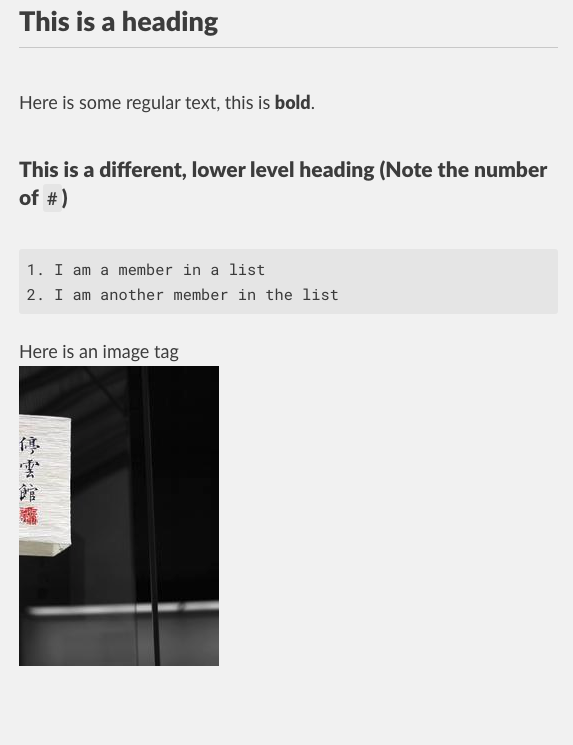
\includegraphics{fig/simple_md.png}

More markdown tags are available, hopefully these give you an idea of how markdown works. Here is a helpful `cheat-sheet' with many more tags you can use, \href{https://www.rstudio.com/wp-content/uploads/2015/02/rmarkdown-cheatsheet.pdf}{RStudio RMarkdown Cheat Sheet}.

\hypertarget{r-markdown}{%
\section{R Markdown}\label{r-markdown}}

R Markdown is an extension of markdown with R mixed in. The markdown syntax is extended using special blocks that contain R code. When it comes to rendering time, the R is run and the results pushed into the rendered document. By mixing these together we get a tool which we can use to get a literate programmed document that can fulfil all our responsibilities.

\begin{figure}
\centering
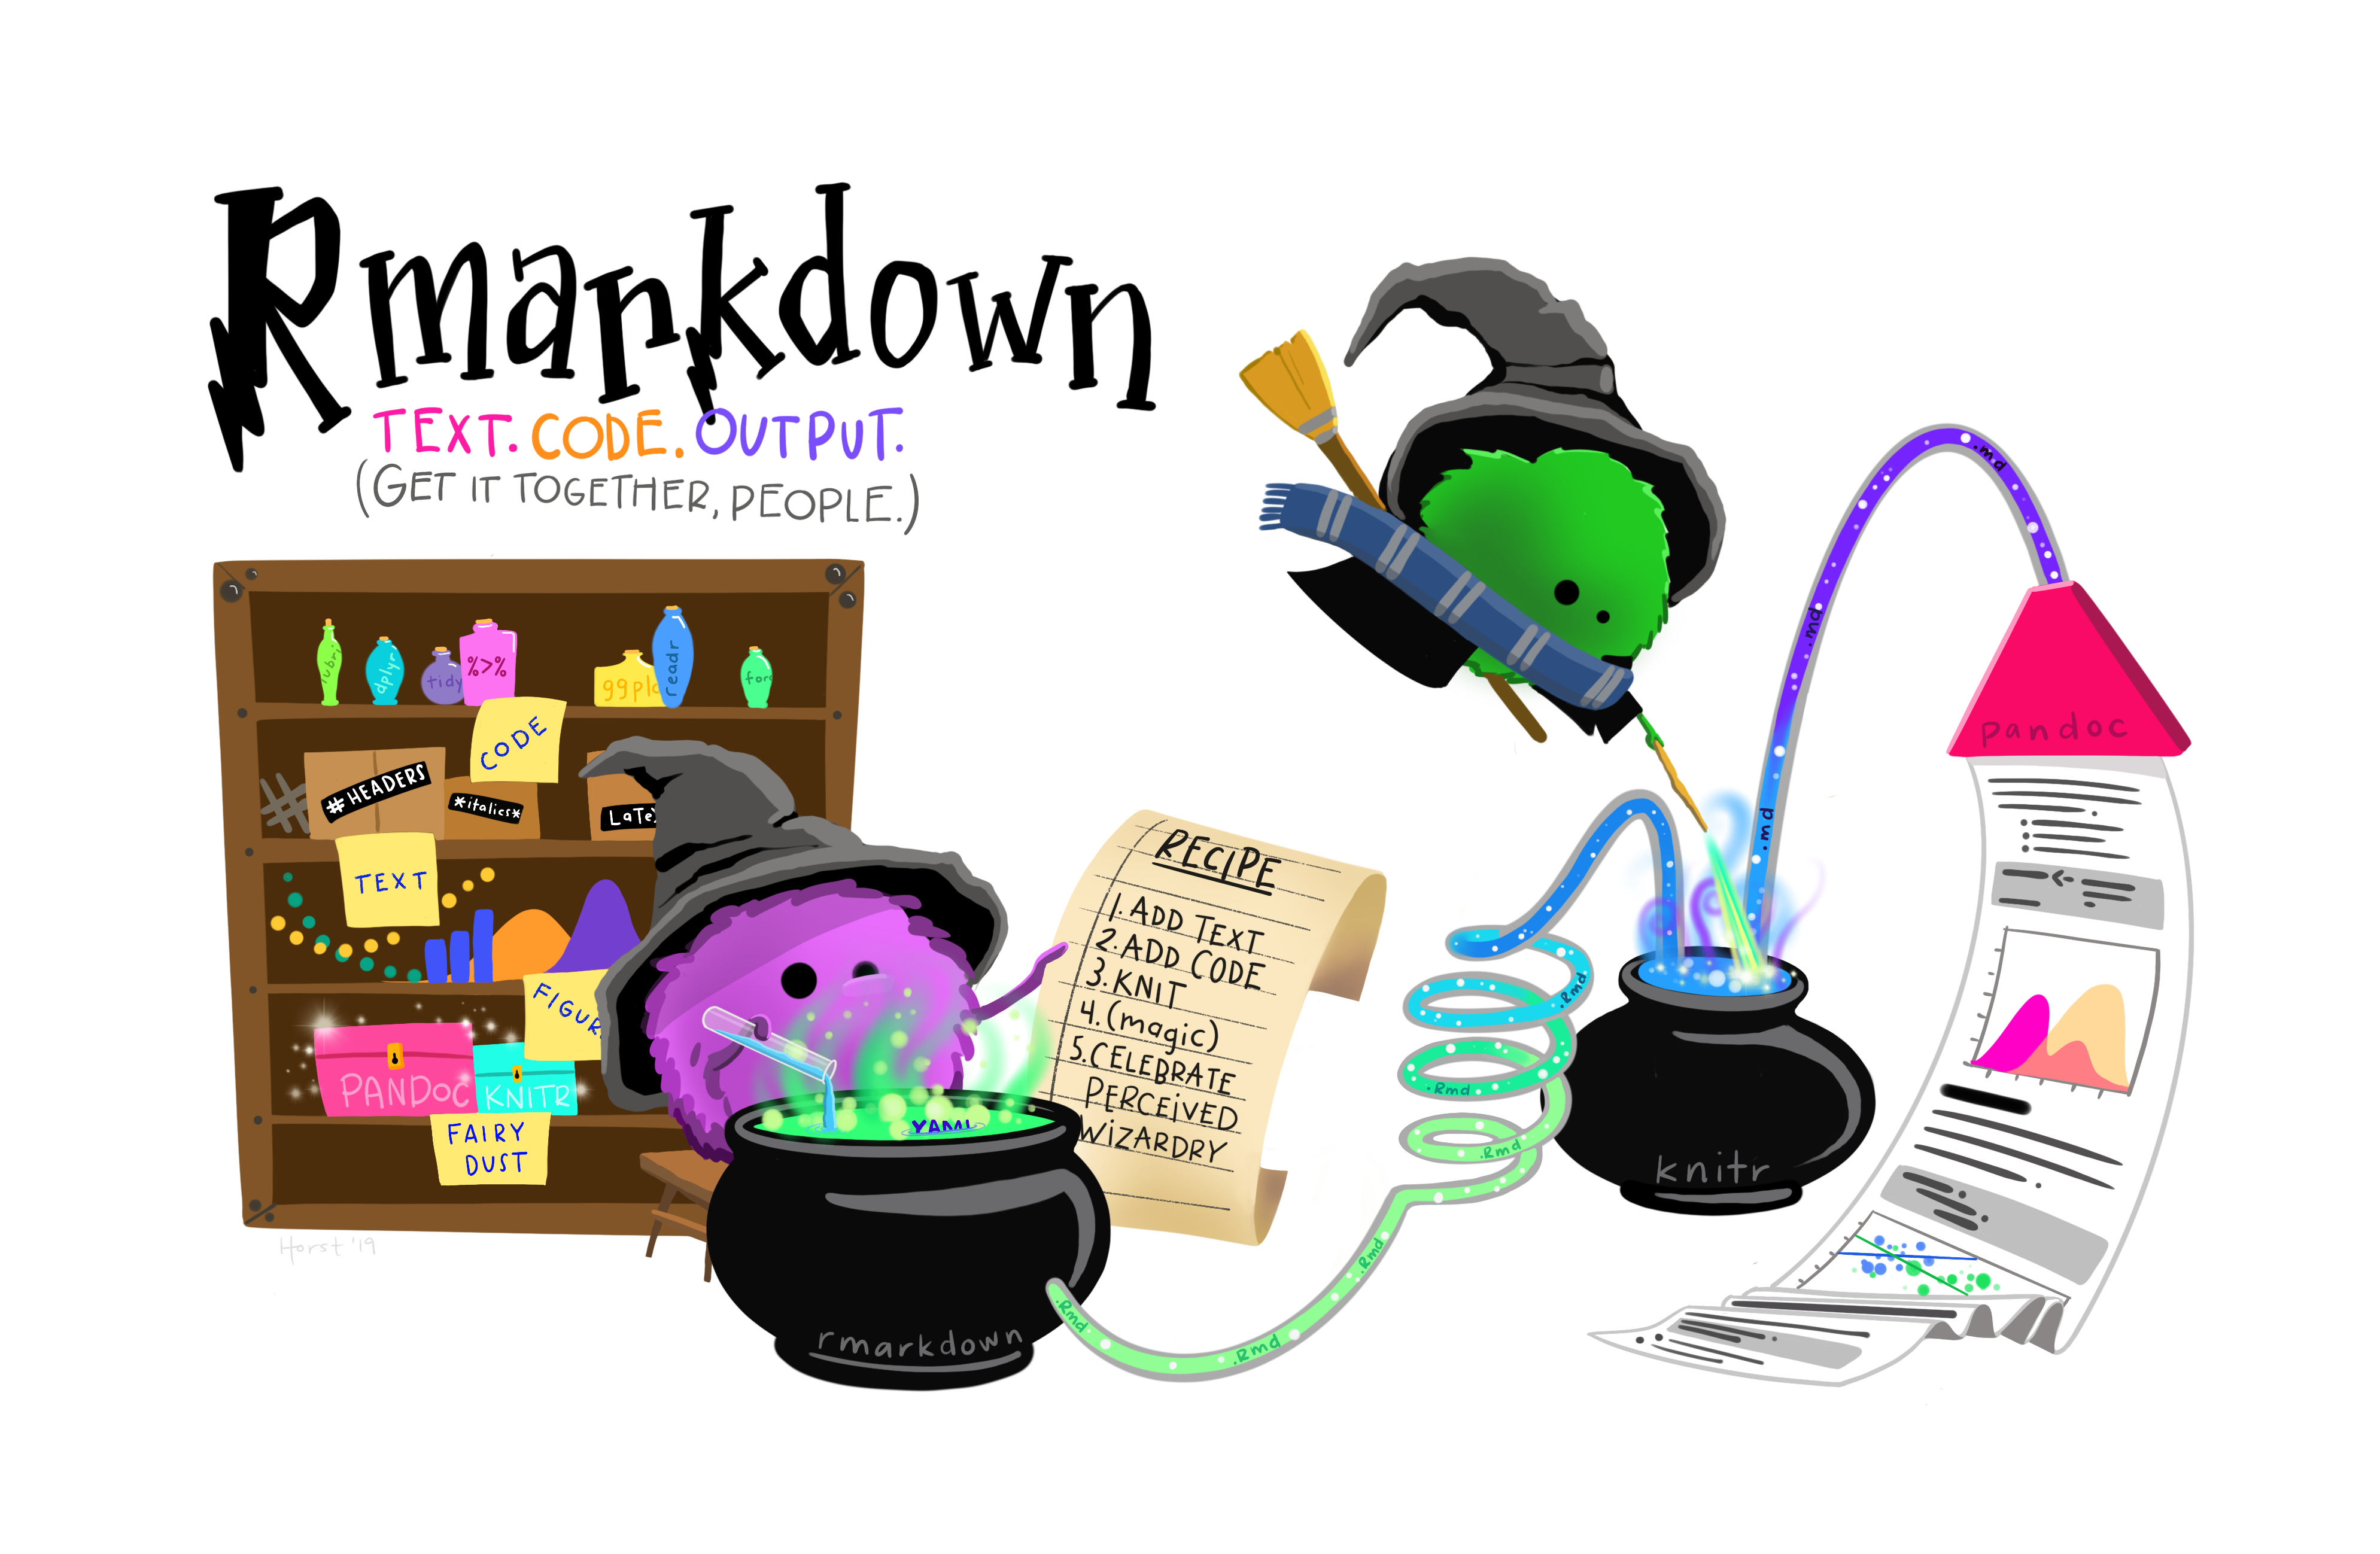
\includegraphics{fig/rmarkdown_wizards.png}
\caption{\label{fig:unnamed-chunk-4}Artwork by \href{https://github.com/allisonhorst}{@AllisonHorst}}
\end{figure}

The R code block we mix in with our regular markdown is structured with \texttt{\textasciigrave{}\textasciigrave{}\textasciigrave{}} (backticks, not quotes) and \texttt{\{r\}}, in practice a block looks like this

\texttt{\textasciigrave{}\textasciigrave{}\textasciigrave{}\{r\}}

\texttt{print("Hello,\ World!")}

\texttt{\textasciigrave{}\textasciigrave{}\textasciigrave{}}

Any R code can go in the blocks, and the program remembers state between blocks so that stuff you do in earlier blocks is remembered in later ones.

\hypertarget{using-r-markdown-in-rstudio}{%
\subsection{Using R Markdown in RStudio}\label{using-r-markdown-in-rstudio}}

RStudio provides a lot of tools for creating RMarkdown documents easily. To get a basic template document you can use the menu's \texttt{File\ -\textgreater{}\ New\ File\ -\textgreater{}\ R\ Markdown}. On doing this you see a dialogue box, usually you want to set the options as in the figure below (you can put your name and a title in the relevant boxes )

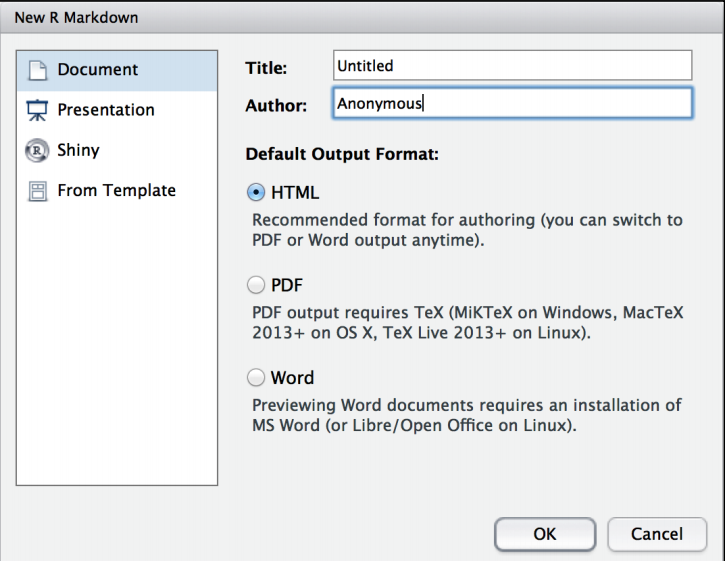
\includegraphics{fig/rmd_dialogue.png}

When you do this you get a new draft document.

\begin{task}
Using RStudio, create a new RMarkdown document. Read it and compare it with what goes below.
\end{task}

\hypertarget{header-information}{%
\subsubsection{Header Information}\label{header-information}}

The first bit of the draft document is a bit of YAML markup that captures some information about the document. You don't need to change anything here if you don't want to, though it can be useful to use the information at this link to set the date automatically \href{https://bookdown.org/yihui/rmarkdown-cookbook/update-date.html}{Dates in RMarkdown}

\begin{verbatim}
---
title: "My Document"
author: "Dan MacLean"
date: "20/04/2021"
output: html_document
---
\end{verbatim}

\hypertarget{setup-block}{%
\subsubsection{Setup Block}\label{setup-block}}

The next part is the automatically created set up block

\begin{verbatim}
`` ```{r setup, include=FALSE} ``
`knitr::opts_chunk$set(echo = TRUE)`
`` ``` ``
\end{verbatim}

This is a standard R block with some options set. The first bit `\texttt{\textasciigrave{}\textasciigrave{}\textasciigrave{}\{r\ setup,\}} is the standard block start, but this one is named \texttt{setup}. You don't need to name each block, but it can be helpful when bugs start to appear. The next bit \texttt{include=FALSE} is an option that tells the RMarkdown renderer \emph{not} to include the code or it's output in the final document, this is because this is just setup code that we don't want messing up our nice output. Then we have the code that this block runs \texttt{knitr::opts\_chunk\$set(echo\ =\ TRUE)} which set up some formatting options. You can use this block for any bits of setup code that you don't want in the rest of your document.

\hypertarget{markdown-and-r-blocks}{%
\subsubsection{Markdown and R blocks}\label{markdown-and-r-blocks}}

The other blocks are the document's standard code and text blocks. Read them then perform this task

\begin{task}
Using RStudio, render the document using the \texttt{Knit} button at the top of the editor pane.
\end{task}

Note how the code and results, including plots are mixed in the resulting document.

\begin{task}
Make some text edits and change the plot titles, then re-knit the document.
\end{task}

\hypertarget{conclusion}{%
\subsection{Conclusion}\label{conclusion}}

This all there really is to RMarkdown documents, they are a very easy to use tool for keeping your analyses readable and reproducible. Inspect the cheat sheet a little further for tips on what more you can do in RMarkdown, \href{https://www.rstudio.com/wp-content/uploads/2015/02/rmarkdown-cheatsheet.pdf}{RStudio RMarkdown Cheat Sheet}.

\begin{roundup}
\begin{verbatim}
* RMarkdown documents are excellent tools for creating readable, attractive and dynamic 
\end{verbatim}

reproducible literate programming documents.
\end{roundup}

\hypertarget{python-and-jupyter-notebooks}{%
\chapter{Python and Jupyter Notebooks}\label{python-and-jupyter-notebooks}}

\hypertarget{about-this-chapter-1}{%
\section{About this chapter}\label{about-this-chapter-1}}

\begin{enumerate}
\def\labelenumi{\arabic{enumi}.}
\tightlist
\item
  Questions

  \begin{itemize}
  \tightlist
  \item
    How do I write a reproducible analysis document in Python with Jupyter??
  \end{itemize}
\item
  Objectives

  \begin{itemize}
  \tightlist
  \item
    Mix markdown and Python with Rmarkdown
  \item
    Run an interactive analysis document
  \end{itemize}
\item
  Keypoints

  \begin{itemize}
  \tightlist
  \item
    Jupyter notebooks are excellent tools for creating readable, attractive and dynamic reproducible literate programming documents.
  \end{itemize}
\end{enumerate}

\hypertarget{jupyter-notebooks}{%
\section{Jupyter Notebooks}\label{jupyter-notebooks}}

A Jupyter Notebook is really quite similar to an RMarkdown document in that it mixes code and markdown in different blocks and allows the user to create a reproducible document. Jupyter varies from RMarkdown slightly in that it prioritises interactive work, instead of rendering a whole document, each block is run individually. Making the whold process a bit more step-by-step than in R Markdown.

\hypertarget{trying-out-jupyter-on-the-web}{%
\section{Trying Out Jupyter on The Web}\label{trying-out-jupyter-on-the-web}}

Because Jupyter notebooks are a bit fiddly to get started, there is an online test notebook set up by the Jupyter authors - \href{https://jupyter.org/try}{Classic Jupyter Notebook}. It can be a bit busy so may take a few reloads to get started.

\begin{task}
\begin{verbatim}
* Go to the link above and start a classic Jupyter notebook. 
* Work through the `Notebook Basics` section.
* Start a new workbook and play around mixing Python Code and Markdown.
* Save as an html file when you are done
\end{verbatim}
\end{task}

\hypertarget{starting-jupyter}{%
\section{Starting Jupyter}\label{starting-jupyter}}

\hypertarget{macos-and-linux}{%
\subsection{macOS and Linux}\label{macos-and-linux}}

To get Jupyter running on your machine, you need to have Python 3, and the \texttt{jupyter} and \texttt{ipython} packages installed. That is all listed in the set up of this course.

Once those are installed you can start a new notebook server by typing \texttt{jupyter\ notebook} at the terminal. Depending on the particulars of your local set up you may need to select an appropriate conda environment beforehand. A new server should start showing the filesystem in your web browser, use the buttons in the web page to start a new notebook.

\hypertarget{windows-1}{%
\subsection{Windows}\label{windows-1}}

There should be a Start Menu item that will let you kick off a new Jupyter notebook server. Simply click on that.

\begin{task}
\begin{verbatim}
* Start a new workbook and play around mixing Python Code and Markdown.
* Pay attention to the block type options dropdown in the interface (under the `Widgets` menu), here is where you can tell the document whether you are writing some Markdown or entering Python. Use the `Run` button to run the code/render the Markdown.  
* Save as an html file when you are done
\end{verbatim}
\end{task}

\begin{roundup}
\begin{verbatim}
* Jupyter Notebooks are excellent tools for creating readable, attractive and dynamic reproducible literate programming documents.
\end{verbatim}
\end{roundup}

\hypertarget{references}{%
\chapter{References}\label{references}}

  \bibliography{book.bib,packages.bib}

\end{document}
